\documentclass[11pt,a4paper]{article}
\usepackage[utf8]{inputenc}
\usepackage{amsmath,amsfonts,amssymb}
\usepackage{graphicx}
\usepackage{geometry}
\geometry{margin=1in}
\usepackage{booktabs}
\usepackage{hyperref}
\usepackage{float}
\usepackage{xcolor}

\title{\textbf{EE3621: Digital Signal Processing} \\ \Large Lecture 26: DSP for Power Systems --- Harmonic Analysis \& Phasor Estimation \\ \large (III B.Tech EEE)}
\author{Lecture Notes (40-Minute Plan)}
\date{}

\definecolor{darkbg}{HTML}{0d121f}
\definecolor{lighttext}{HTML}{e2e8f0}
\definecolor{primary}{HTML}{8b5cf6}
\definecolor{secondary}{HTML}{0dd5c5}

\pagecolor{darkbg}
\color{lighttext}

\hypersetup{
    colorlinks=true,
    linkcolor=secondary,
    urlcolor=secondary
}

\begin{document}

\maketitle

\section{Lecture Plan (40 Minutes Breakdown)}
\begin{itemize}
    \item \textbf{00:00 -- 05:00 (5 mins):} Power Quality Issues, Harmonics, THD.
    \item \textbf{05:00 -- 12:00 (7 mins):} Fourier Analysis of Power Signals, DFT.
    \item \textbf{12:00 -- 17:00 (5 mins):} DFT Spectral Leakage and mitigation.
    \item \textbf{17:00 -- 22:00 (5 mins):} Phasor Measurement Units (PMUs), TVE.
    \item \textbf{22:00 -- 27:00 (5 mins):} Recursive (Sliding) DFT.
    \item \textbf{27:00 -- 32:00 (5 mins):} Kalman Filter for Phasor Tracking.
    \item \textbf{32:00 -- 35:00 (3 mins):} Protection Relay DSP \& Anti-Aliasing.
    \item \textbf{35:00 -- 40:00 (5 mins):} Active/Reactive Power from DFT \& Checkpoints.
\end{itemize}

\noindent\rule{\textwidth}{0.5pt}

\section{Power Quality Issues}
Nonlinear loads (VFDs, UPS, rectifiers) draw non-sinusoidal currents. The Total Harmonic Distortion (THD) quantifies this:
\begin{equation}
THD_V = \frac{\sqrt{\sum_{k=2}^N V_k^2}}{V_1}
\end{equation}
High THD causes motor overheating, transformer derating, and capacitor bank failures.

\section{Fourier Analysis of Power Signals}

\begin{figure}[H]
    \centering
    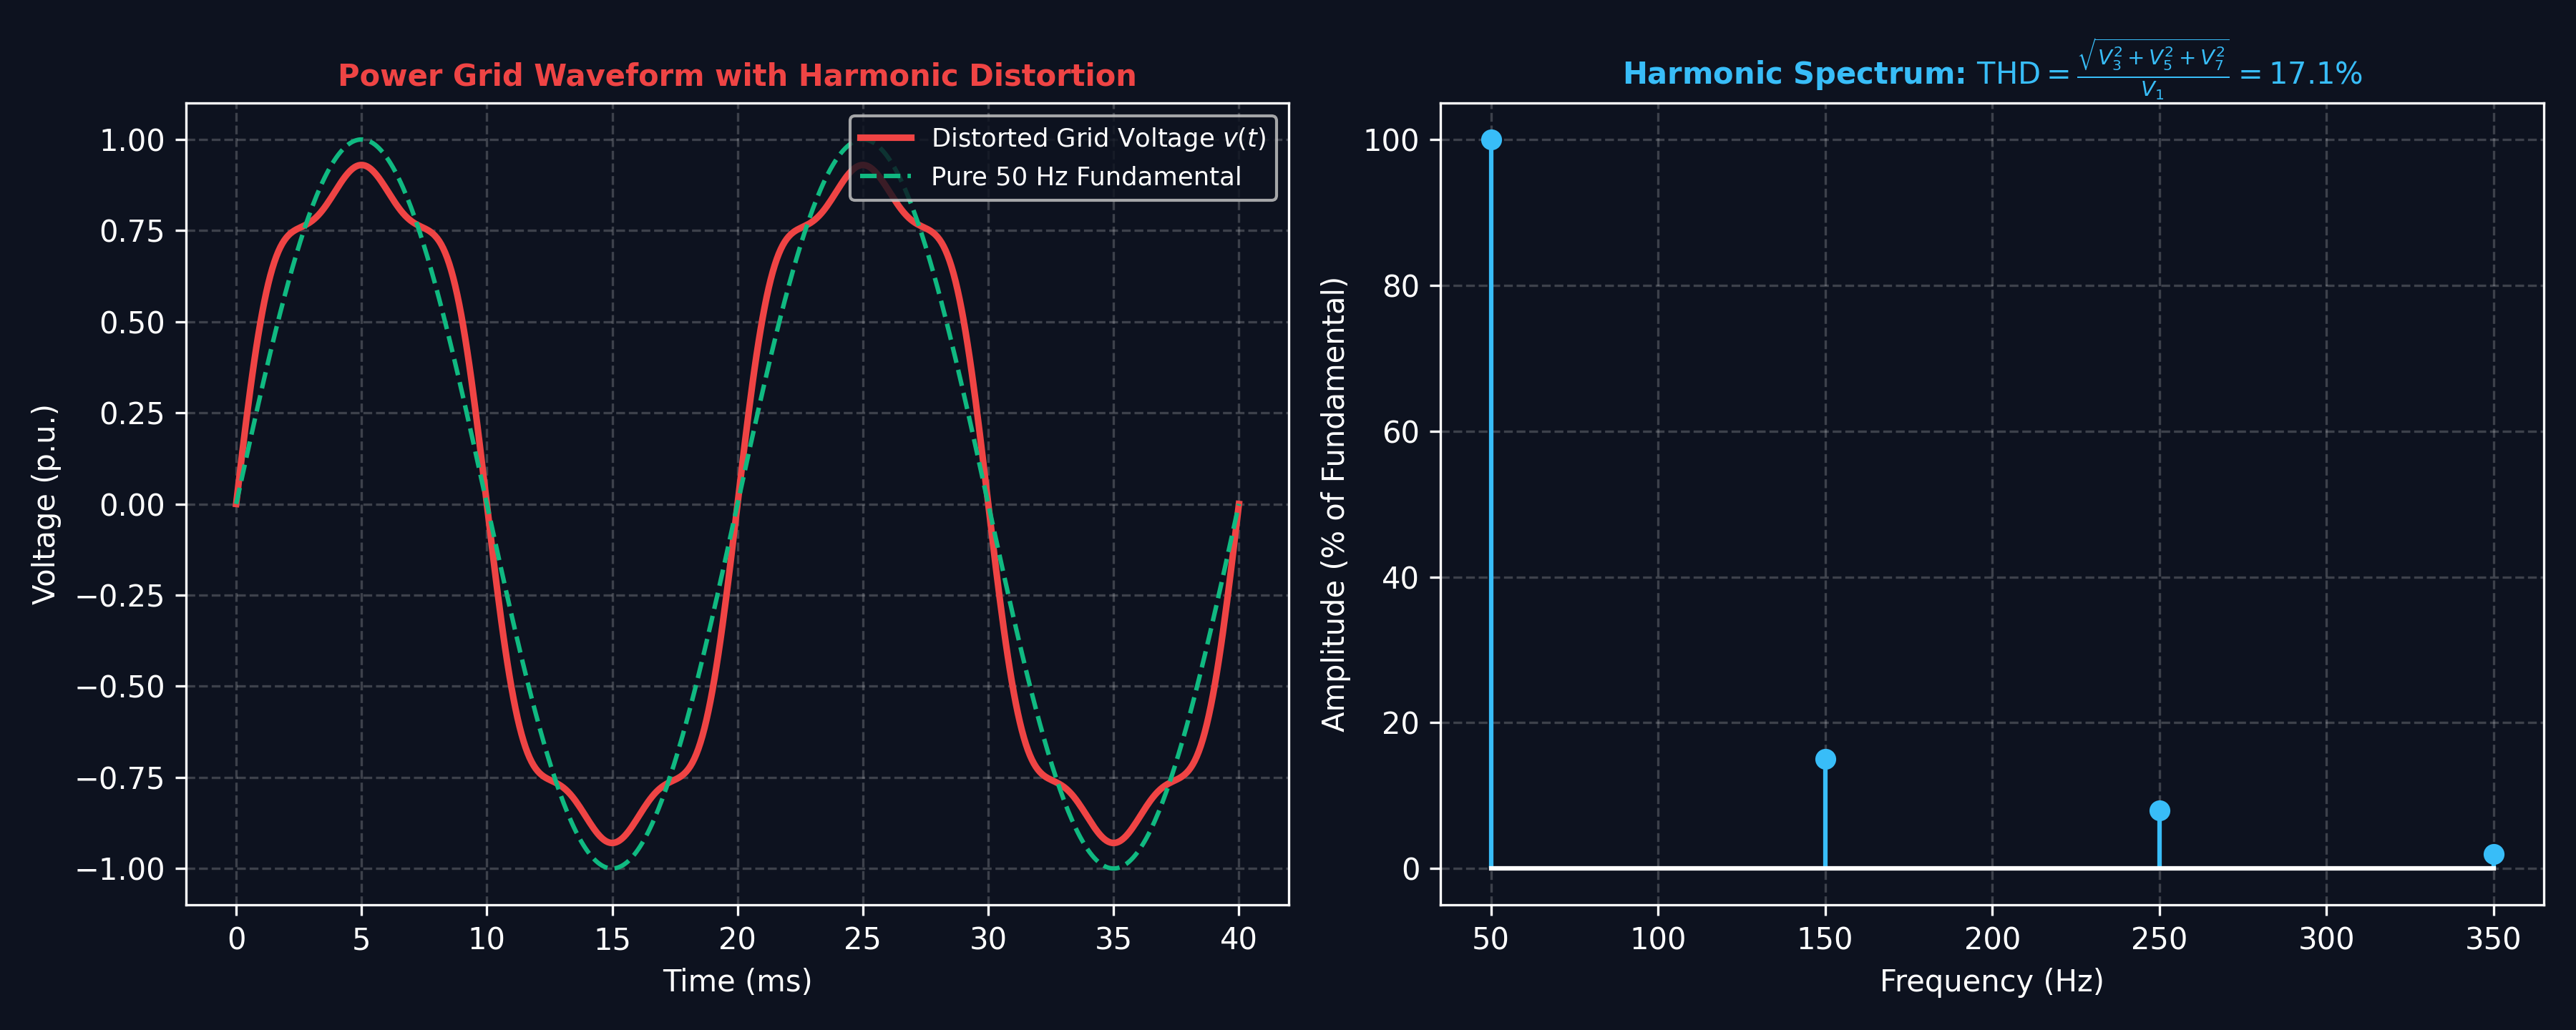
\includegraphics[width=0.85\textwidth]{images/power_harmonics_waveform_thd.png}
    \caption{Power Grid Voltage Distortion and Harmonic Spectrum with Total Harmonic Distortion (THD) Calculation.}
\end{figure}

\begin{figure}[H]
    \centering
    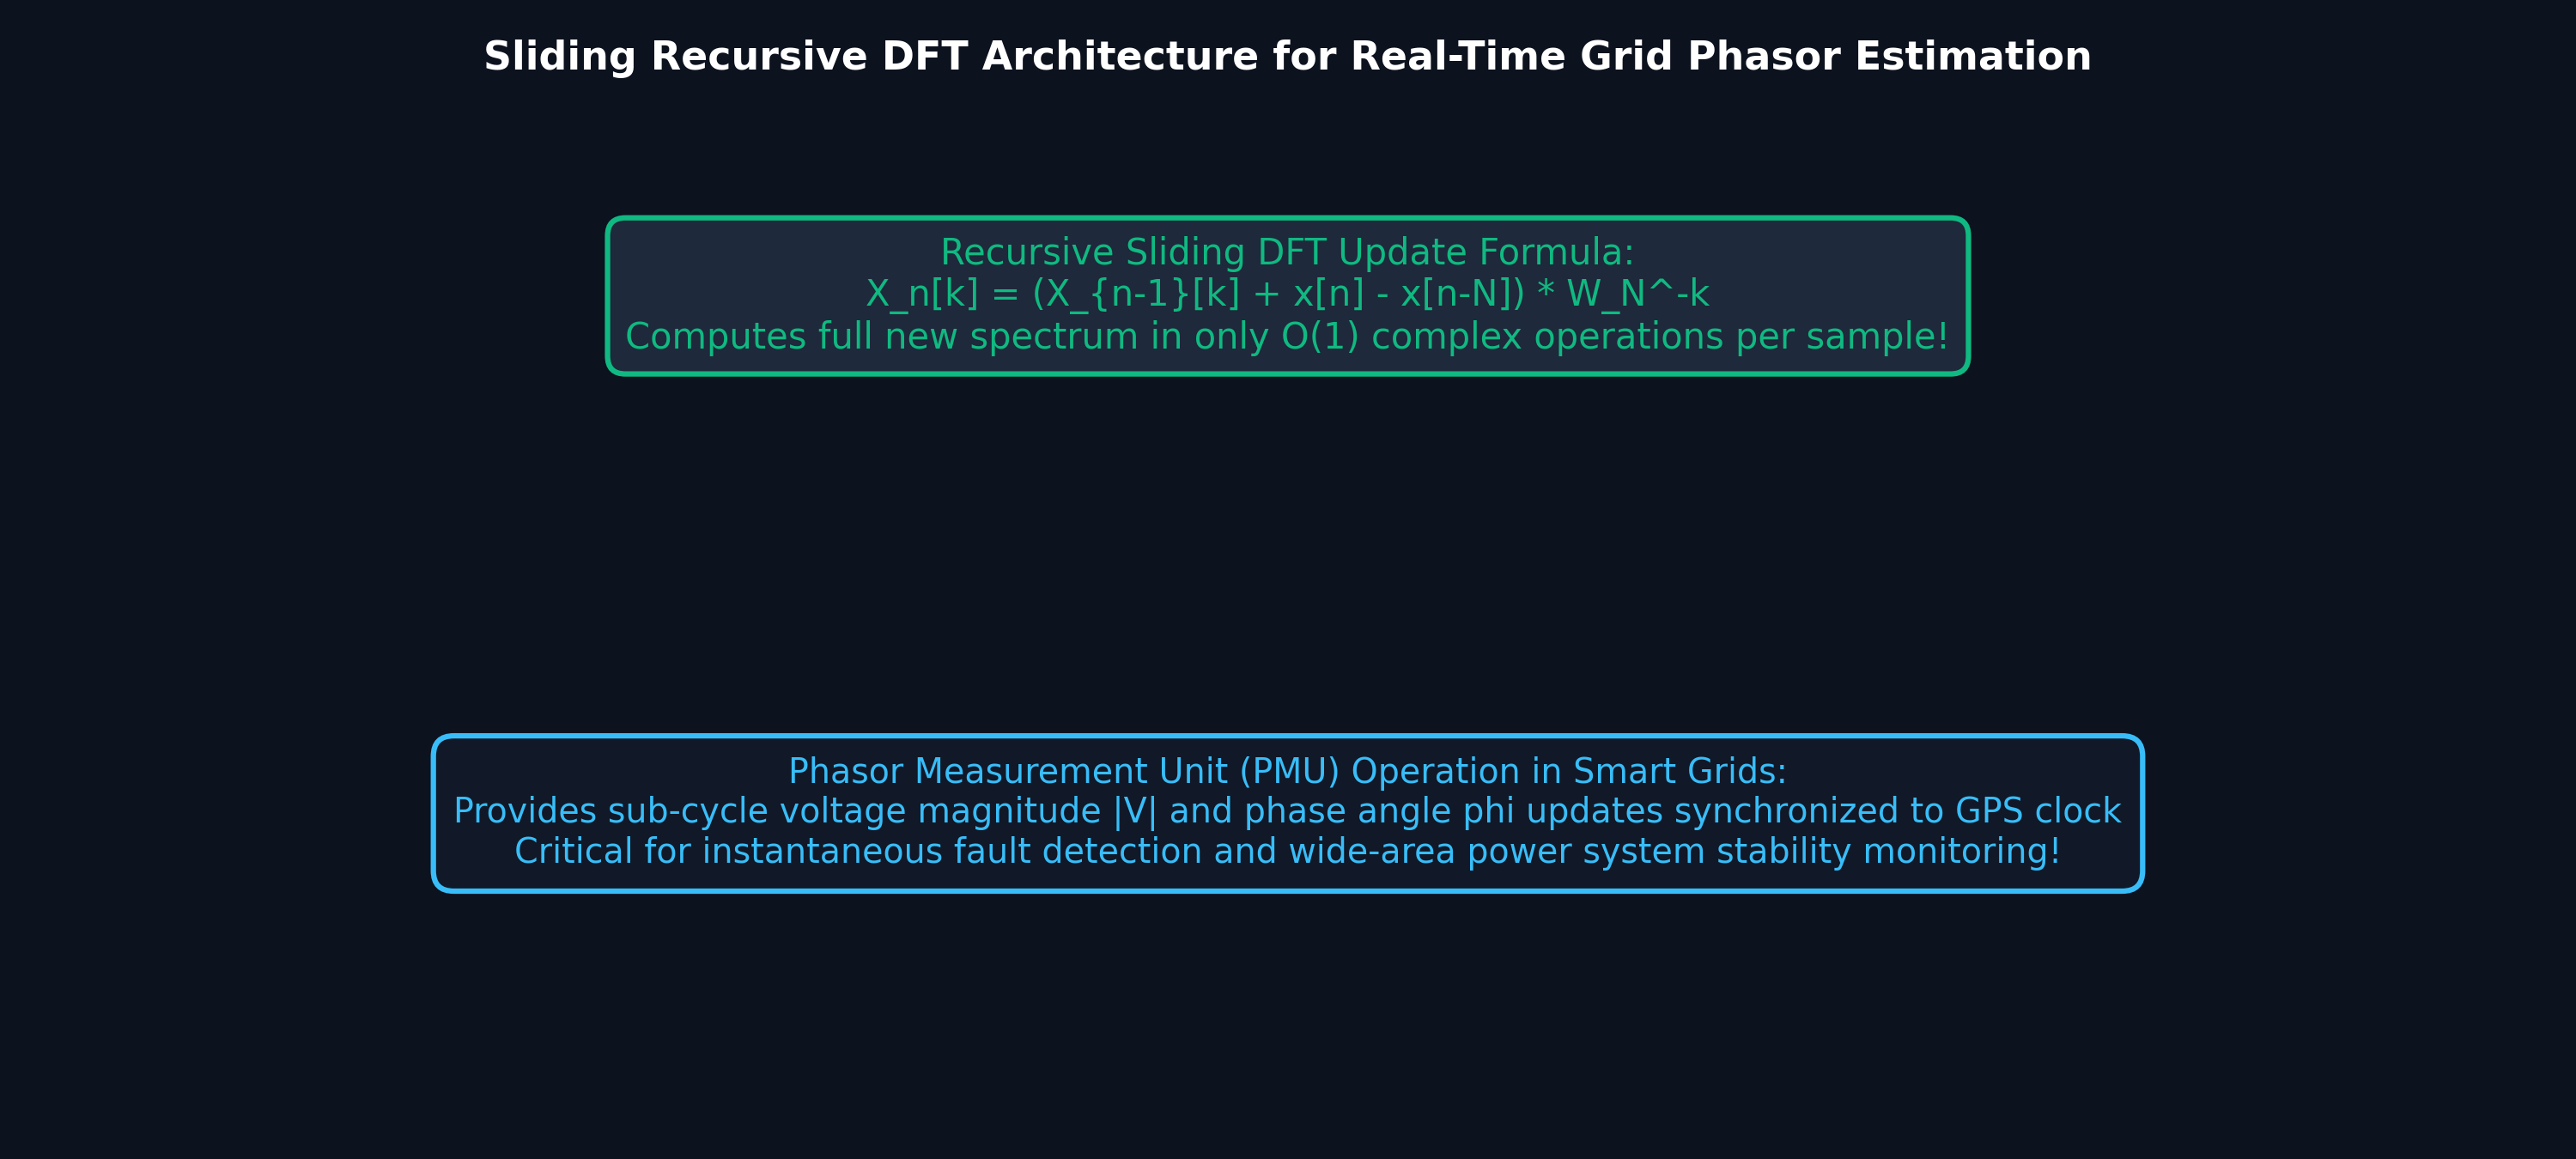
\includegraphics[width=0.85\textwidth]{images/sliding_dft_phasor_tracking.png}
    \caption{Recursive Sliding-DFT Architecture for Real-Time GPS-Synchronized Phasor Measurement Units (PMUs).}
\end{figure}


The fundamental frequency $f_0 = 50/60$ Hz is sampled at $f_s$, requiring an integer number of samples per cycle $N = f_s / f_0$. The DFT yields complex harmonic phasors:
\begin{equation}
V_k = \frac{2}{N} \sum_{n=0}^{N-1} x[n] e^{-j \frac{2\pi}{N} k n}
\end{equation}

\section{DFT Leakage in Power Systems}
When $f_0$ drifts (e.g., to $49.8$ Hz), the $N$-sample window no longer perfectly spans one cycle. This non-integer cycle lengths cause spectral leakage. Mitigation involves windowing and interpolation-based frequency estimation.

\section{Phasor Measurement Units (PMUs)}
Synchrophasors are time-synchronized by GPS (1-PPS). The IEEE C37.118 standard requires the Total Vector Error (TVE) to be strictly less than $1\%$:
\begin{equation}
\text{Phasor} = \frac{V_{peak}}{\sqrt{2}} e^{j\phi}
\end{equation}
\begin{equation}
\text{TVE} = \sqrt{ \frac{(\hat{X}_r - X_r)^2 + (\hat{X}_i - X_i)^2}{X_r^2 + X_i^2} } \times 100\%
\end{equation}

\section{Recursive DFT (Sliding DFT)}
To track real-time phasors efficiently, we update the DFT sample-by-sample. 
Derivation:
\begin{align}
X_k[n] &= \sum_{m=0}^{N-1} x[n-m] W_N^{k(N-1-m)} \\
X_k[n] &= \left( X_k[n-1] - x[n-N]W_N^0 + x[n]W_N^{kN} \right) W_N^{-k} \\
X_k[n] &= \left( X_k[n-1] + x[n] - x[n-N] \right) e^{j \frac{2\pi}{N} k}
\end{align}
This reduces computation from $O(N \log N)$ for a full FFT to $O(1)$ per harmonic per sample.

\section{Kalman Filter for Phasor Tracking}
The state model uses phasor amplitude and phase as states, and noisy voltage samples as measurements.
\begin{align}
\mathbf{x}_k &= \mathbf{x}_{k-1} + \mathbf{w}_k \\
z_k &= \mathbf{H}_k \mathbf{x}_k + v_k
\end{align}
where $\mathbf{H}_k = [ \cos(k \theta_0) \quad -\sin(k \theta_0) ]$.

\section{Protection Relay DSP}
Overcurrent, distance, and differential relays use DFT-based phasor estimation. Anti-aliasing filters are designed to cutoff below the Nyquist frequency.
Analog lowpass prototypes for these anti-aliasing filters are shown in the figures below.

\section{Active and Reactive Power from DFT}
\begin{align}
P &= \frac{1}{2}\sum_k |V_k||I_k|\cos(\phi_{Vk}-\phi_{Ik}) \\
Q &= \frac{1}{2}\sum_k |V_k||I_k|\sin(\phi_{Vk}-\phi_{Ik})
\end{align}

\section{Checkpoint Questions}
\begin{enumerate}
    \item \textbf{THD Calculation:} Calculate THD given $V_1=230, V_3=40, V_5=30$.
    \\ \textit{Answer:} $THD_V = \frac{\sqrt{40^2+30^2}}{230} = 21.74\%$.
    \item \textbf{Samples per Cycle:} For $f_s=2880$ Hz and $f_0=60$ Hz, $N=48$. The 5th harmonic (300 Hz) corresponds to $k=5$.
    \item \textbf{Recursive DFT Efficiency:} Recursive updates require just 1 complex multiplication per step, compared to $O(N \log N)$ for a full FFT.
\end{enumerate}

\end{document}
